\documentclass{article}
\usepackage[utf8]{inputenc}
\usepackage{amsmath}
\usepackage{graphicx}
\usepackage{xcolor}
\usepackage{caption}
\usepackage[margin=1in]{geometry}

% ----------------------------------------------------------------------

\title{Applied Statistics Problem Set}
\author{Student name}
\date{3rd of January 2021}

\begin{document}

\maketitle

I have worked with student A (All problems), student B (problem 1.2) and student C (problem 1.3).


%%%%%%%%%%%%%%%% PART I %%%%%%%%%%%%%%%%%%%%%%%%%%%%%%%%%%%%%%%%%%%%%%%
\section*{I - Distributions and probabilities}

This is a template for the problem set and exam hand in for Applied Statistics. Please submit one pdf file with your solutions, with answers \textbf{\underline{bolded and underlined}} where relevant.
%
All tables and figures should be easy to read and clearly referenced. There's no page limit, but it should be possible to keep it under 10-15 pages, especially if you want the TAs to stay happy!
%
There is no need to submit or show any code (unlike for the exam, where this should be submitted separately), just your answers. Finally, please state who you worked with at the top of the report, but remember that your answers should be your own.


\subsection*{Problem 1.1} You can add sub sections for questions here. 

\subsubsection*{1.1.1} $N_3$ follows X distribution, since...

\subsubsection*{1.1.2} The probability can be calculated as follows...


% ----------------------------------------------------------------------
\subsection*{1.2}
More answers here. 



%%%%%%%%%%%%%%%% PART II %%%%%%%%%%%%%%%%%%%%%%%%%%%%%%%%%%%%%%%%%%%%%%%
\section*{II - Error Propagation}
You can add equations, like so, in Equation \ref{eq1}: 

\begin{equation}
    \chi ^{2} = \sum \frac{(model-data)^{2}}{error^{2}}
    \label{eq1}
\end{equation}

\subsection*{Problem 2.1}
\subsubsection*{2.1.1} The uncertainty...



%%%%%%%%%%%%%%%% PART III %%%%%%%%%%%%%%%%%%%%%%%%%%%%%%%%%%%%%%%%%%%%%%%
\section*{III - Monte Carlo}
You can add figures, like so, in Figure \ref{fig1} (they may not go exactly where you want - that's alright). 

\begin{figure}[h]
    \centering
    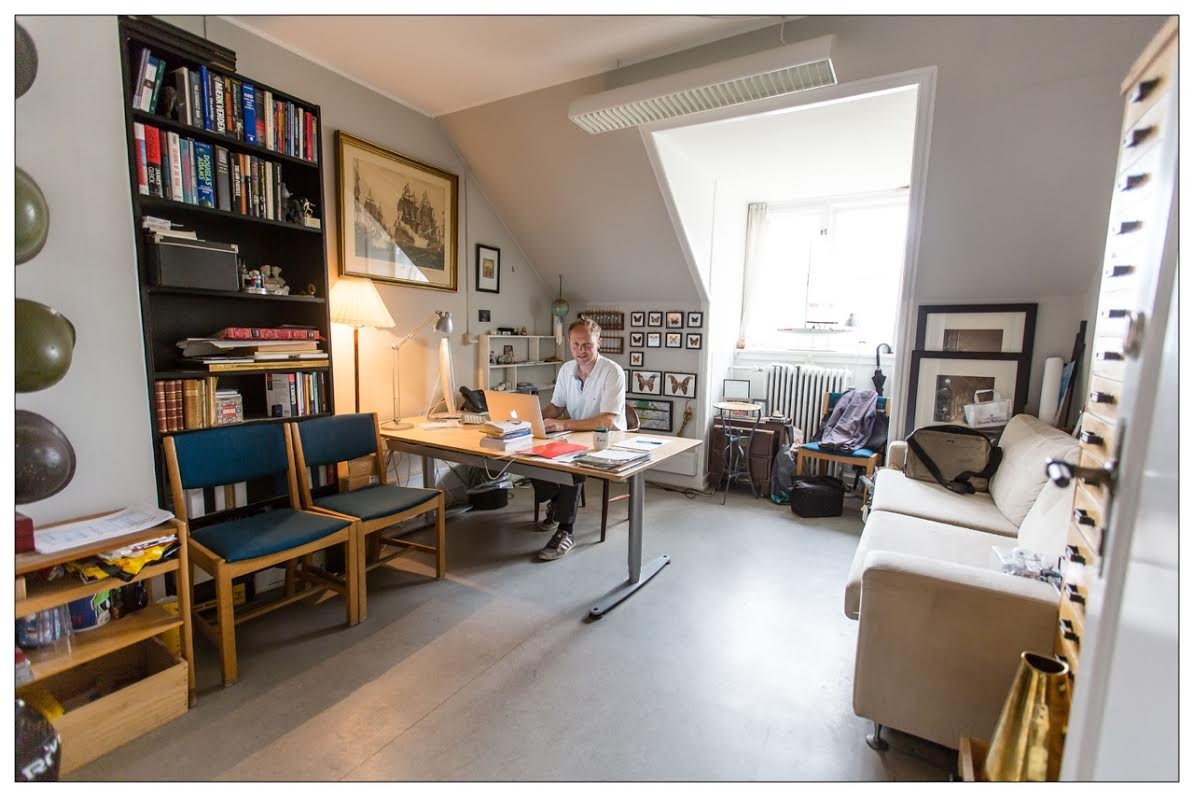
\includegraphics[scale=0.25]{Troels_InOffice.jpg}
    \caption{``A friendly man'' [Katriona Gould]}
    \label{fig1}
\end{figure}

\section*{Problem 3.1}
You can also create Tables, like so: 

\begin{table}[hbtp!]
\begin{centering}
\begin{tabular}{ |c|c|c|c| } 
  \hline
  Data & $\mu$ & $\sigma$ & N\\ 
  \hline 
  \textbf{Data1} & 0.0 & 1.0 & 100 \\ 
  \textbf{Data2} & 0.0 & 1.0 & 100 \\ 
  \hline
\end{tabular}
\caption{Mean ($\mu$), standard deviation ($\sigma$) and data set length (N) for two different data sets.}
\label{tab:cleaned}
\end{centering}
\end{table}

Finally, it makes for easier reading, if you include colors, for example between \textcolor{red}{sample A} and \textcolor{blue}{sampel B}, but that is of course just an option.



%%%%%%%%%%%%%%%% PART III %%%%%%%%%%%%%%%%%%%%%%%%%%%%%%%%%%%%%%%%%%%%%%%
\section*{III - Monte Carlo}

%%%%%%%%%%%%%%%% PART IV %%%%%%%%%%%%%%%%%%%%%%%%%%%%%%%%%%%%%%%%%%%%%%%
\section*{IV - Statistical tests}

%%%%%%%%%%%%%%%% PART V %%%%%%%%%%%%%%%%%%%%%%%%%%%%%%%%%%%%%%%%%%%%%%%
\section*{V - Fitting data}


%%%%%%%%%%%%%%%% Bibliography %%%%%%%%%%%%%%%%%%%%%%%%%%%%%%%%%%%%%%%%%%%%%%%
\bibliography{}
%Roger Barlow: Statistics: A guide to the use of statistics.

\end{document}
